\documentclass[compress]{beamer}
\usepackage{ifthen,verbatim,ulem}

\title{``Slow'' Refitting of TeV Muon Showers}
\author{Jim Pivarski}
\institute{Texas A\&M University}
\date{16 October, 2008}

\newcommand{\isnote}{}
\xdefinecolor{lightyellow}{rgb}{1.,1.,0.25}
\xdefinecolor{darkblue}{rgb}{0.1,0.1,0.7}

%% Uncomment this to get annotations
%% \def\notes{\addtocounter{page}{-1}
%%            \renewcommand{\isnote}{*}
%% 	   \beamertemplateshadingbackground{lightyellow}{white}
%%            \begin{frame}
%%            \frametitle{Notes for the previous page (page \insertpagenumber)}
%%            \itemize}
%% \def\endnotes{\enditemize
%% 	      \end{frame}
%%               \beamertemplateshadingbackground{white}{white}
%%               \renewcommand{\isnote}{}}

%% Uncomment this to not get annotations
\def\notes{\comment}
\def\endnotes{\endcomment}

\setbeamertemplate{navigation symbols}{}
\setbeamertemplate{headline}{\mbox{ } \hfill
\begin{minipage}{5.5 cm}
\vspace{-0.75 cm} \small
\end{minipage} \hfill
\begin{minipage}{4.5 cm}
\vspace{-0.75 cm} \small
\begin{flushright}
\ifthenelse{\equal{\insertpagenumber}{1}}{}{Jim Pivarski \hspace{0.2 cm} \insertpagenumber\isnote/\pageref{numpages}}
\end{flushright}
\end{minipage}\mbox{\hspace{0.2 cm}}\includegraphics[height=1 cm]{../cmslogo} \hspace{0.1 cm} \includegraphics[height=1 cm]{../tamulogo} \hspace{0.01 cm} \vspace{-1.05 cm}}

\begin{document}
\frame{\titlepage}

%% \begin{notes}
%% \item This is the annotated version of my talk.
%% \item If you want the version that I am presenting, download the one
%% labeled ``slides'' on Indico (or just ignore these yellow pages).
%% \item The annotated version is provided for extra detail and a written
%% record of comments that I intend to make orally.
%% \item Yellow notes refer to the content on the {\it previous} page.
%% \item All other slides are identical for the two versions.
%% \end{notes}

\small

\begin{frame}
\frametitle{The Problem}

\begin{itemize}\setlength{\itemsep}{0.1 cm}
\item TeV muons shower, making it difficult to identify which hits
  belong to the muon and which belong to the delta rays
\item We try dropping bad hits from tracks to improve the resolution:
  FirstStation, Picky, and Cocktail algorithms
\item But we have no mechanism to add hits--- no ability to recover from
  an earlier mistake
\item More rigorous treatment would return to the whole RecHit collection
  for TeV candidates and spend more time to find the best set
\item For example, segment-finding might pick the wrong side of a DT
  hit in a very crowded environment; can be better resolved when we know
  more about the full track
\end{itemize}

\begin{center}
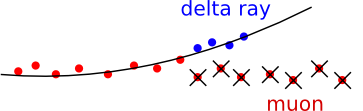
\includegraphics[width=0.5\linewidth]{delta_ray_mistake.png} \hfill 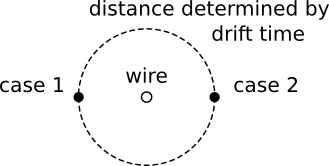
\includegraphics[width=0.4\linewidth]{dt_ambiguity.png}
\end{center}

%% \hspace{-0.83 cm} \textcolor{darkblue}{\Large Outline2}
\end{frame}

\begin{frame}
\frametitle{Slow refitting algorithm}

\begin{itemize}\setlength{\itemsep}{0.35 cm}
\item Consider a new track-refitting algorithm which also revisits hit selection from scratch.  Algorithm must be:

\vspace{0.1 cm}
\hspace{0.5 cm} 1. accurate

\hspace{0.5 cm} \sout{2. fast} \hspace{0.1 cm} \textcolor{darkblue}{No!}

\item Only need to refit rare muons in massive dimuon-pair events

\item We can afford to spend more CPU time at the highest energies \\ in the offline analysis

\item With infinite time, we could try every combination of hits

\[ \big( \mbox{ \#hits per layer } \big)^{ \mbox{ \#layers } } \approx \mbox{ billions of combinations }\]

\item We can almost certainly find the optimum in a more directed search with about 1 minute/muon or less
\end{itemize}
\end{frame}

\begin{frame}
\frametitle{Algorithm details}

\begin{enumerate}
\item Starting with tracker track (assume no showering in tracker),
  make a tree of possible extensions into the muon system
\begin{itemize}
\item At each layer, create a new branch for every possible decision:
  one for each hit, and one for no hit ($>$ 1 hit/layer not allowed)

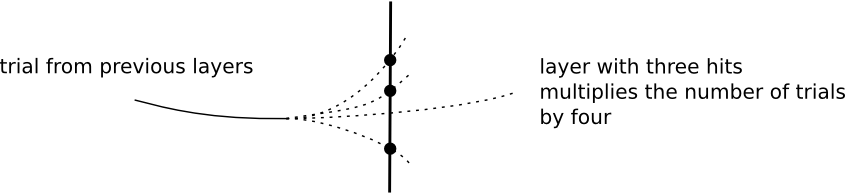
\includegraphics[width=\linewidth]{trial_multiplication.png}

\item $\displaystyle \mbox{score} = \frac{\sum \chi^2_i + N_{\mbox{\scriptsize missing hits}} \times \mbox{missing hit penalty}}{N_{\mbox{\scriptsize layers}}} $

\end{itemize}

\item Sort trials by score, prune branches with too-high \mbox{scores at each layer\hspace{-1 cm}}

\item Completely refit the best 100 or so (to get forward-backward
  smoothed $\chi^2$s), publish the winning trial as the refitted track
\end{enumerate}

Analogy with game theory: from tree of all possible moves, consider only those that lead to winning end-states

\end{frame}

\begin{frame}
\frametitle{Speed optimization}

Unlike a game, our opponent isn't trying to trick us

Trials that start to go bad don't improve (because they're \mbox{following delta rays)\hspace{-1 cm}}

\vfill
\begin{columns}
\column{0.6\linewidth}

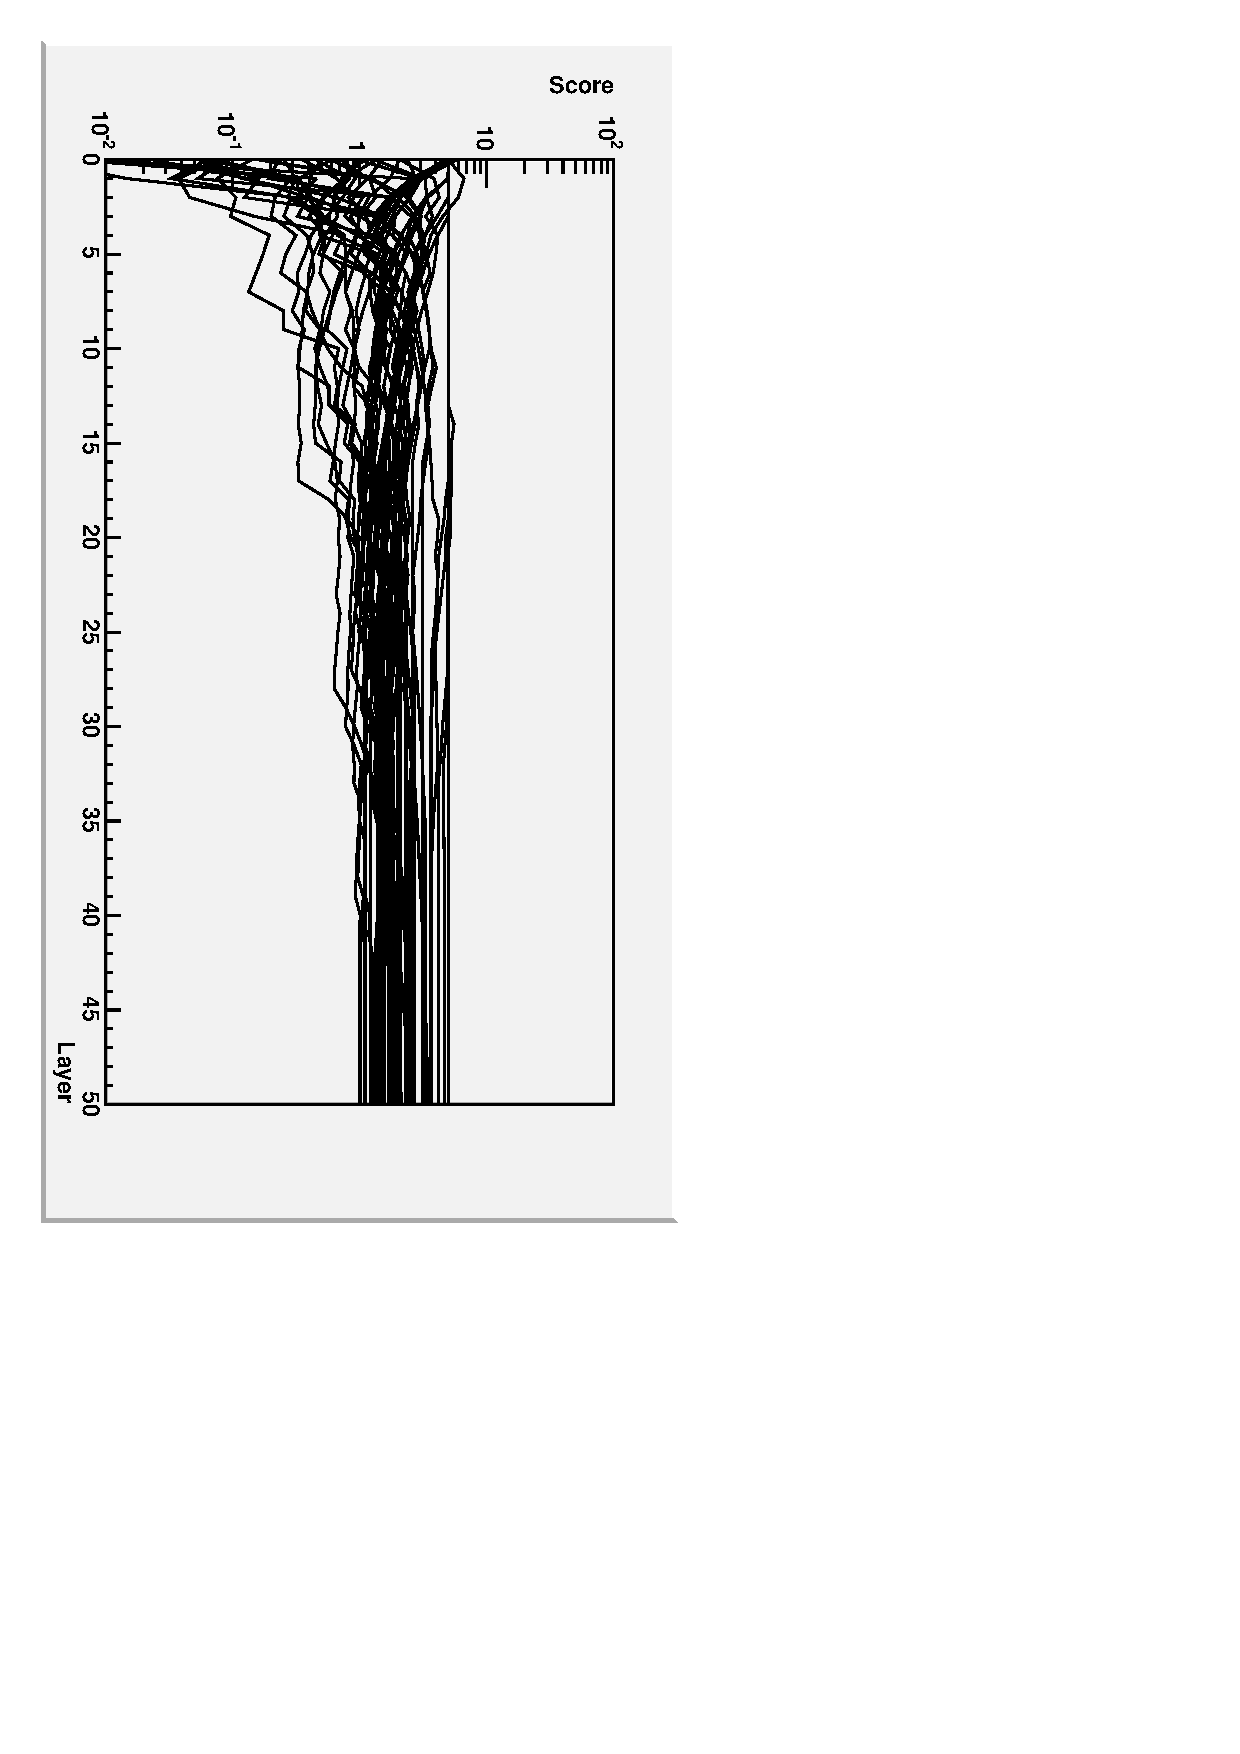
\includegraphics[height=\linewidth, angle=90]{vslayer_score.pdf}

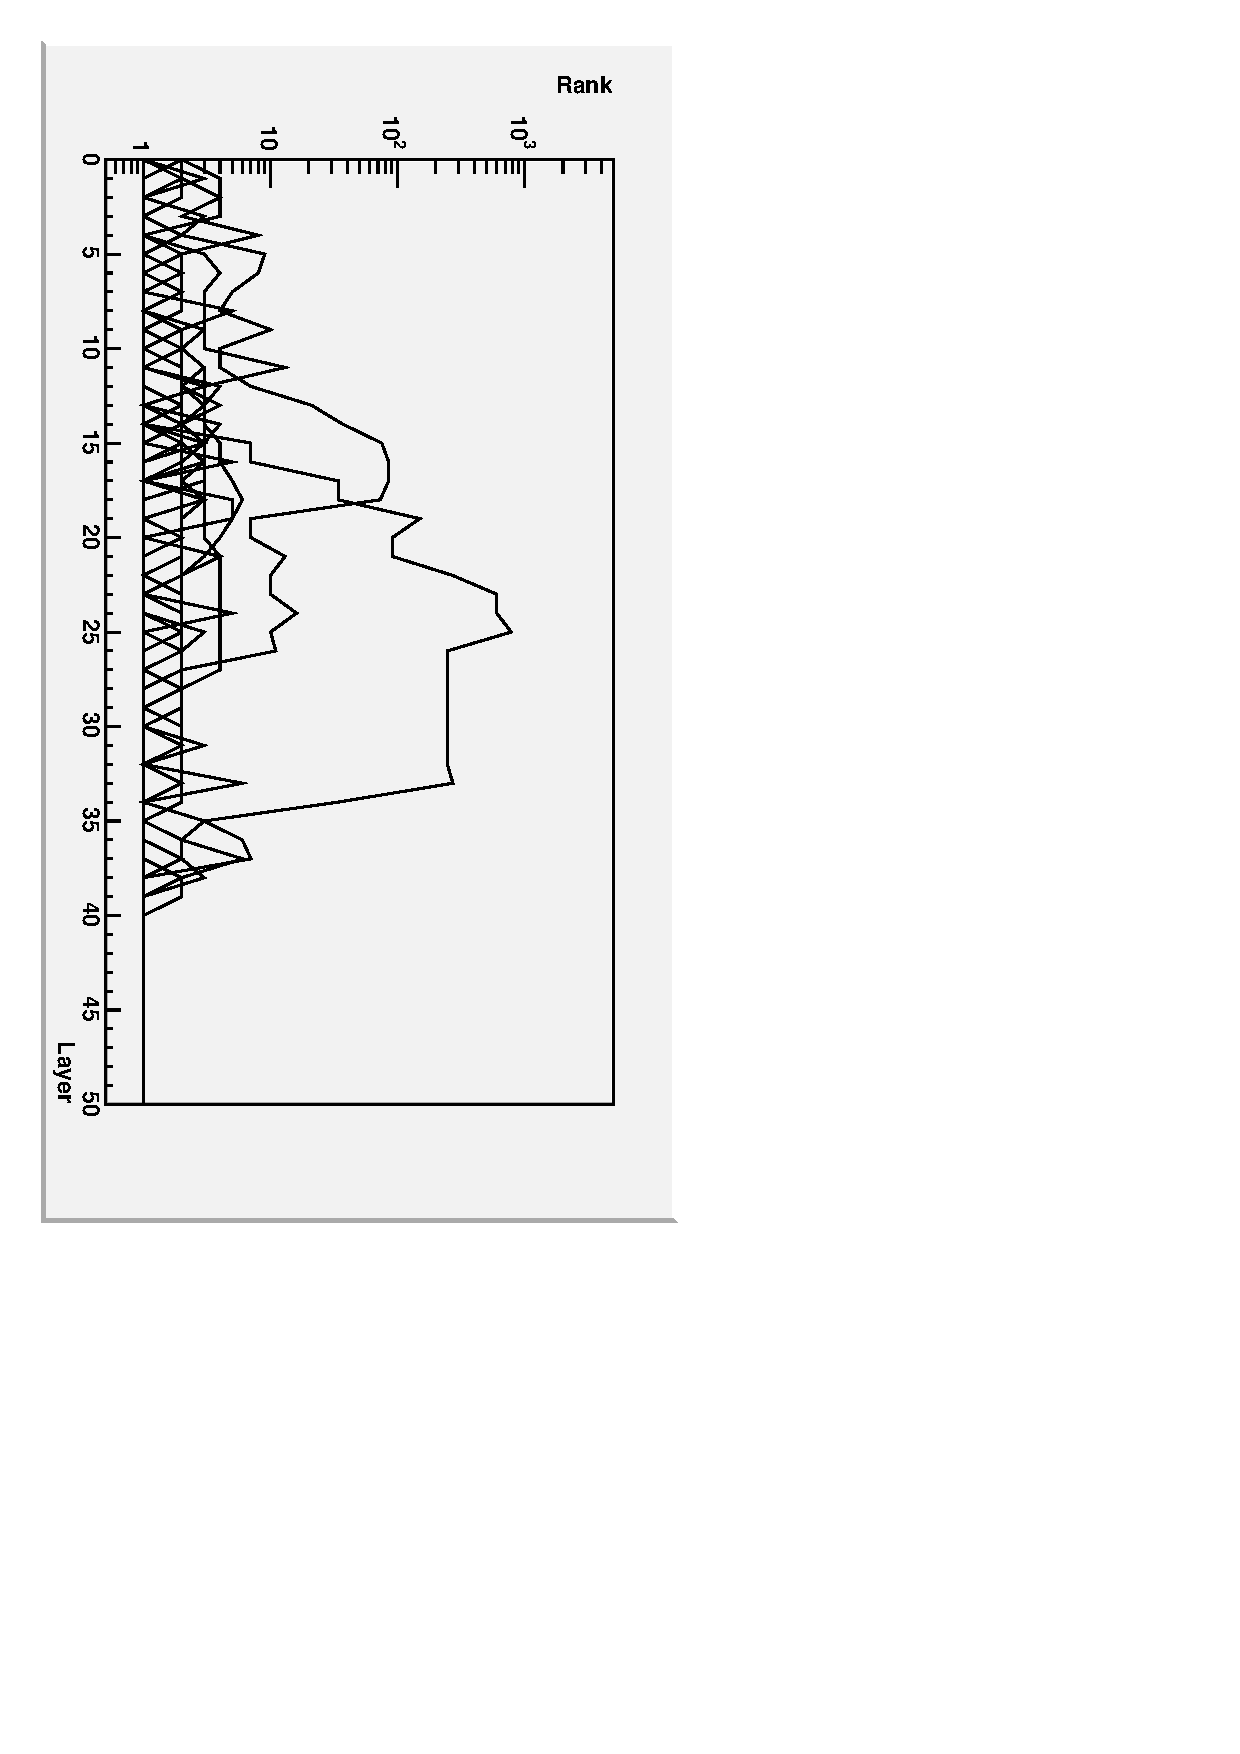
\includegraphics[height=\linewidth, angle=90]{vslayer_rank.pdf}

\column{0.4\linewidth}

\begin{itemize}\setlength{\itemsep}{0.2 cm}
\item Among 50 trials that eventually won, score (reduced $\chi^2$)
  never got above 10

$\longrightarrow$ apply a cut at 100

\item They were always in the top 1000

$\longrightarrow$ cut at 10,000

\item Cut on rank stabilizes running time

\end{itemize}

with these cuts: \mbox{48 sec/muon\hspace{-1 cm}}

\end{columns}

\end{frame}

\begin{frame}
\frametitle{Performance tests: $\chi^2/N_{\mbox{\scriptsize dof}}$}

\begin{itemize}
\item 1000-event sample of 2~TeV $Z'\to\mu\mu$ in 2\_1\_9 (private sample)
\item Use Picky as a baseline for comparison
\item This is the real track $\chi^2$, not score; peak is closer to 1.0, smaller tail
\end{itemize}

\vfill
\begin{columns}
\column{0.5\linewidth}
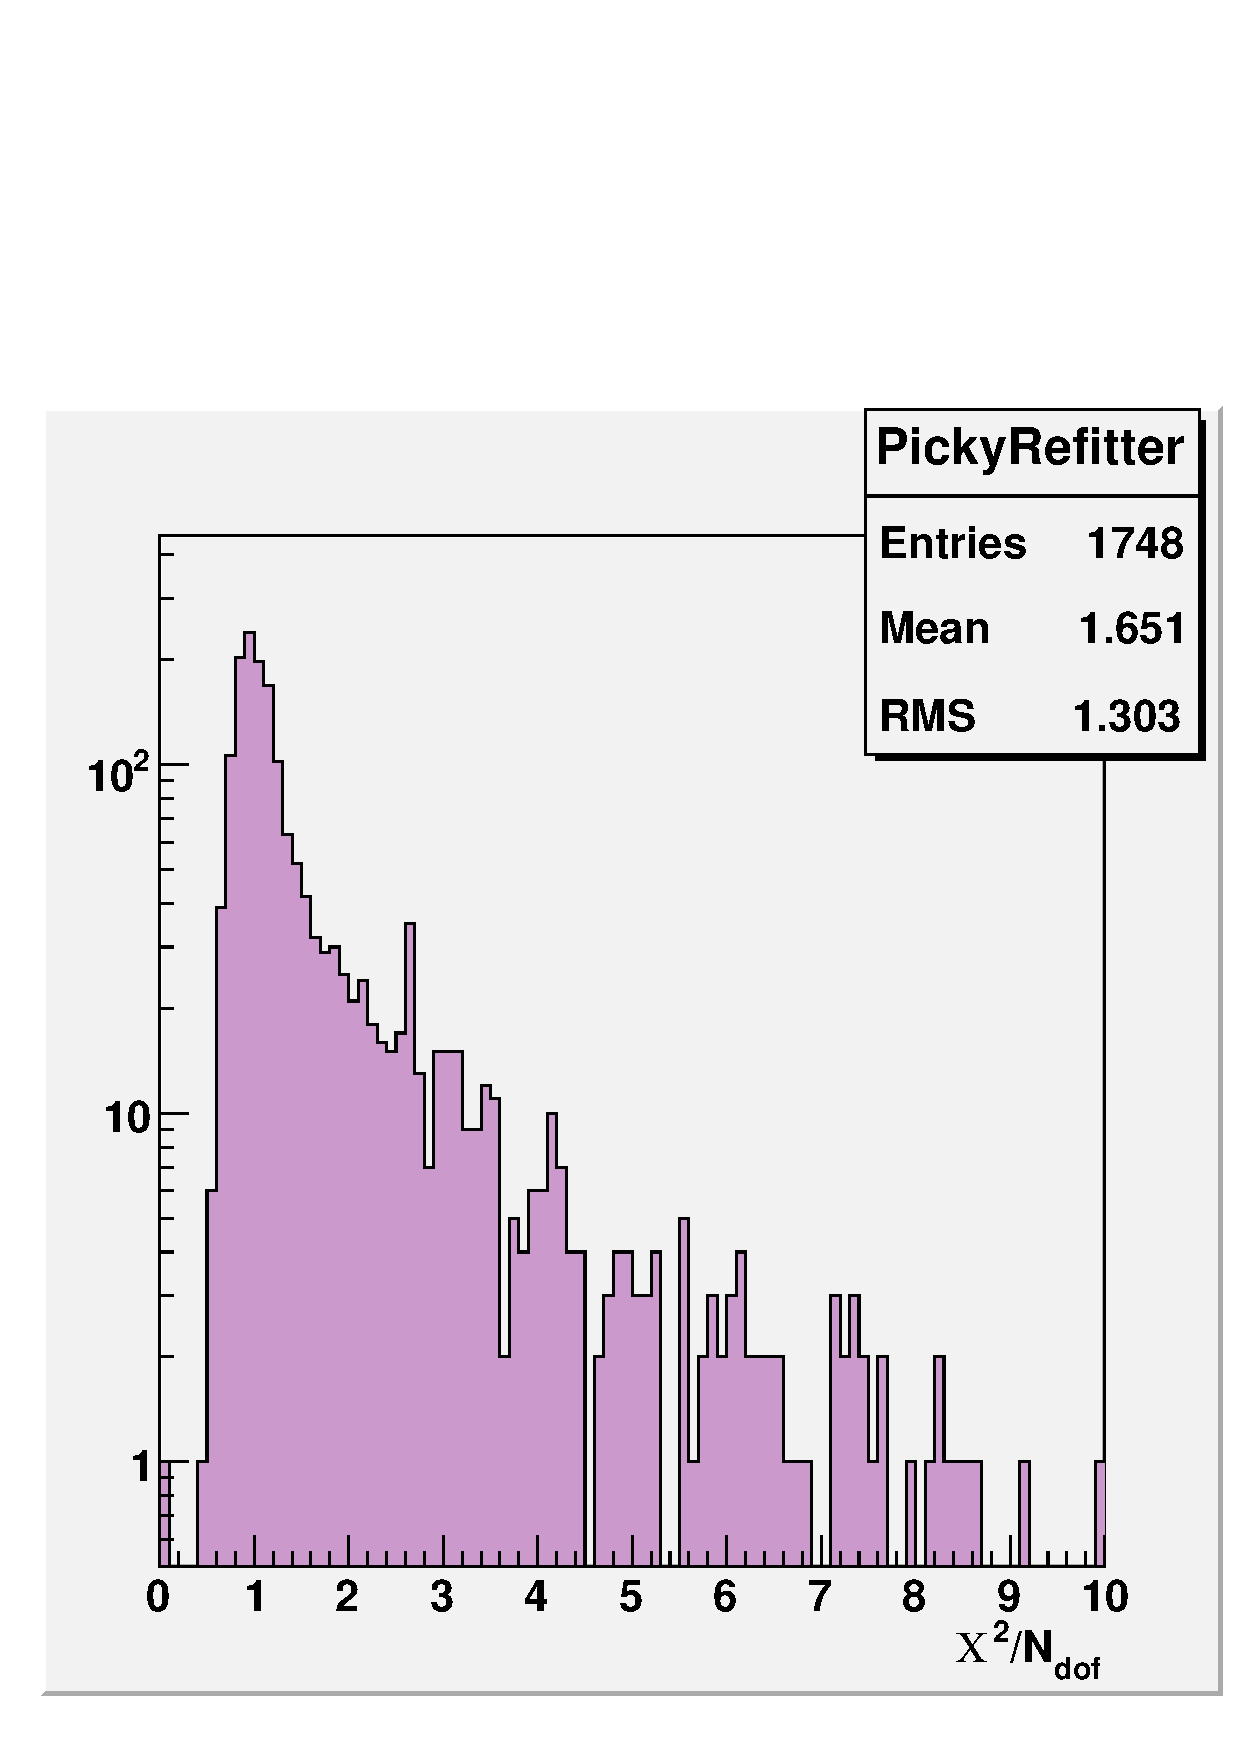
\includegraphics[width=\linewidth]{chi2_picky.pdf}
\column{0.5\linewidth}
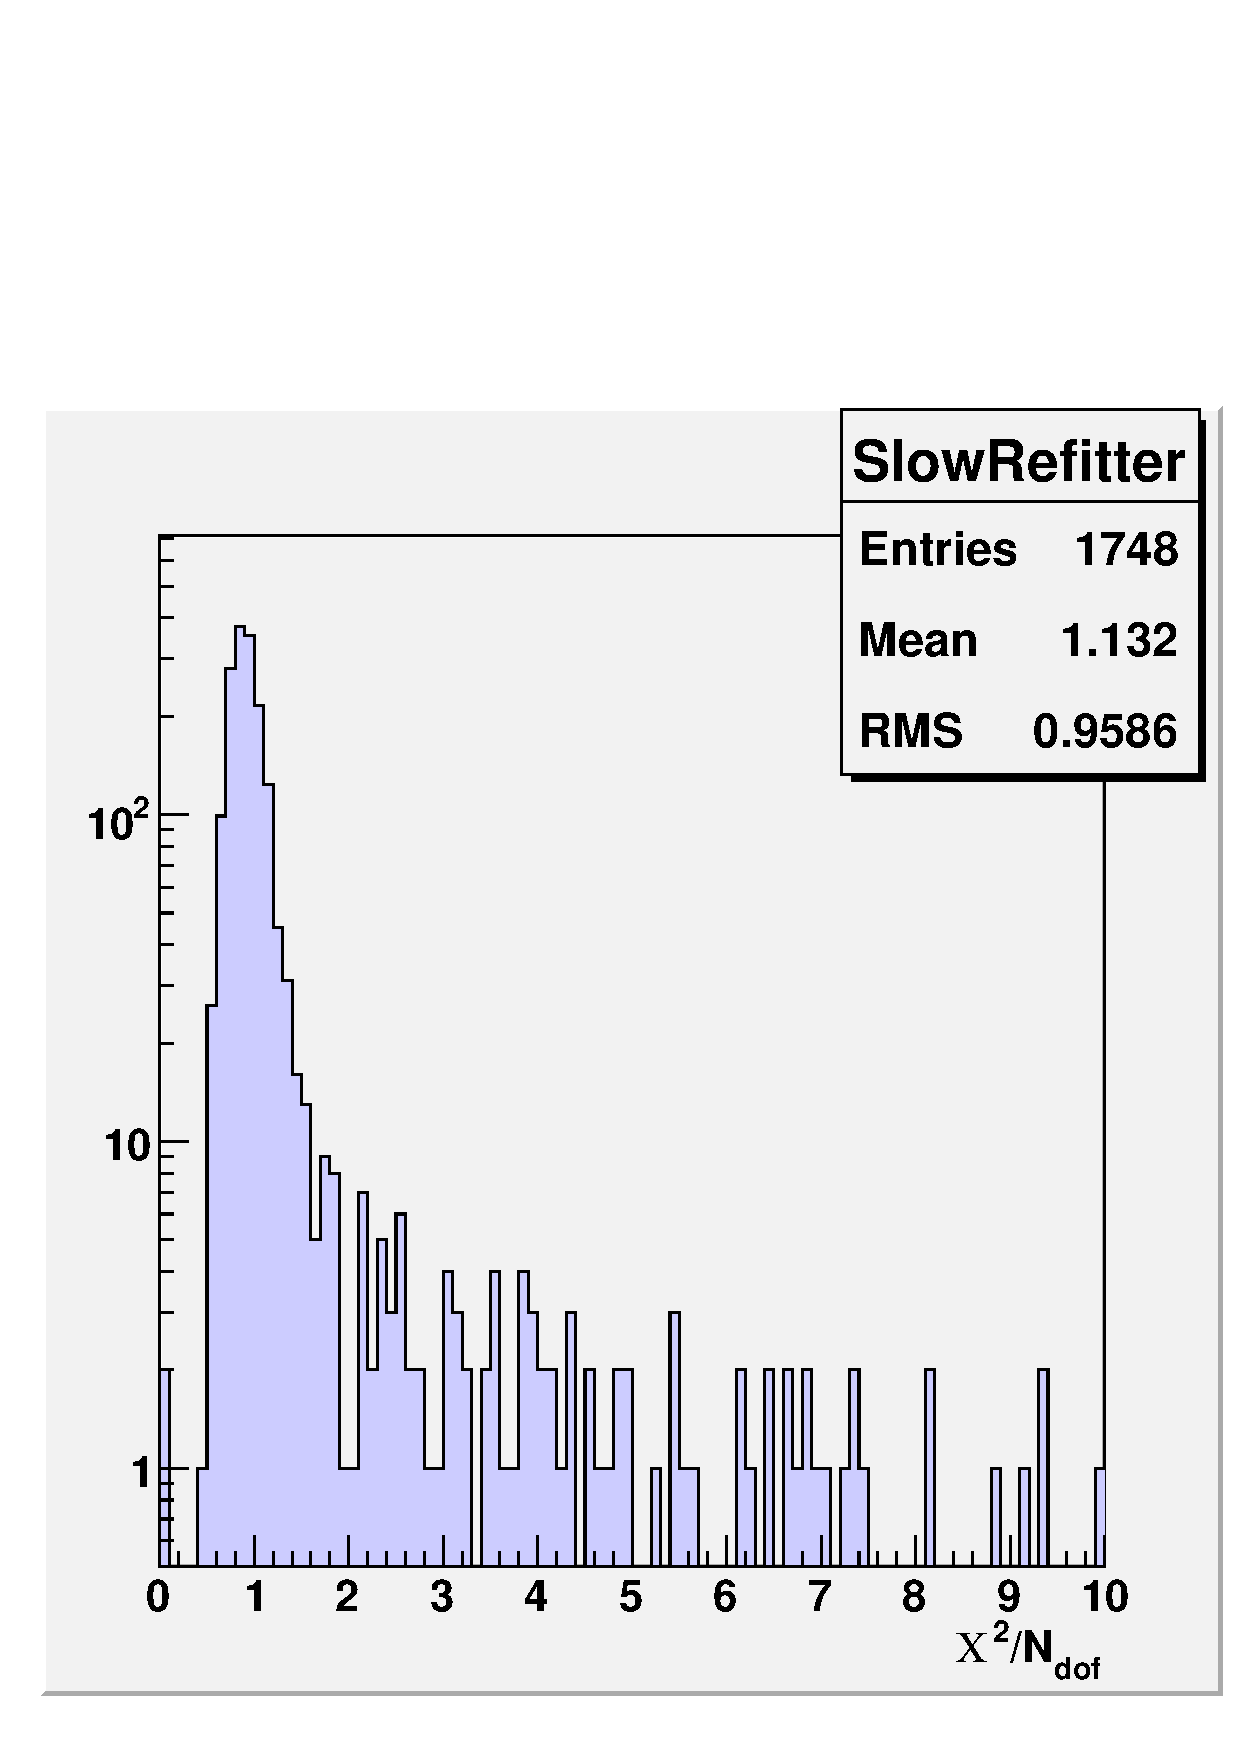
\includegraphics[width=\linewidth]{chi2_slow.pdf}
\end{columns}

\end{frame}

\begin{frame}
\frametitle{Performance tests: \#hits}

\begin{itemize}
\item It is not reducing $\chi^2$ by throwing away more hits
\item Missing hit penalty = 5, unoptimized

Could be made rigorous by converting hit efficiencies into $(\#\sigma)^2$
\end{itemize}

\vfill
\begin{columns}
\column{0.5\linewidth}
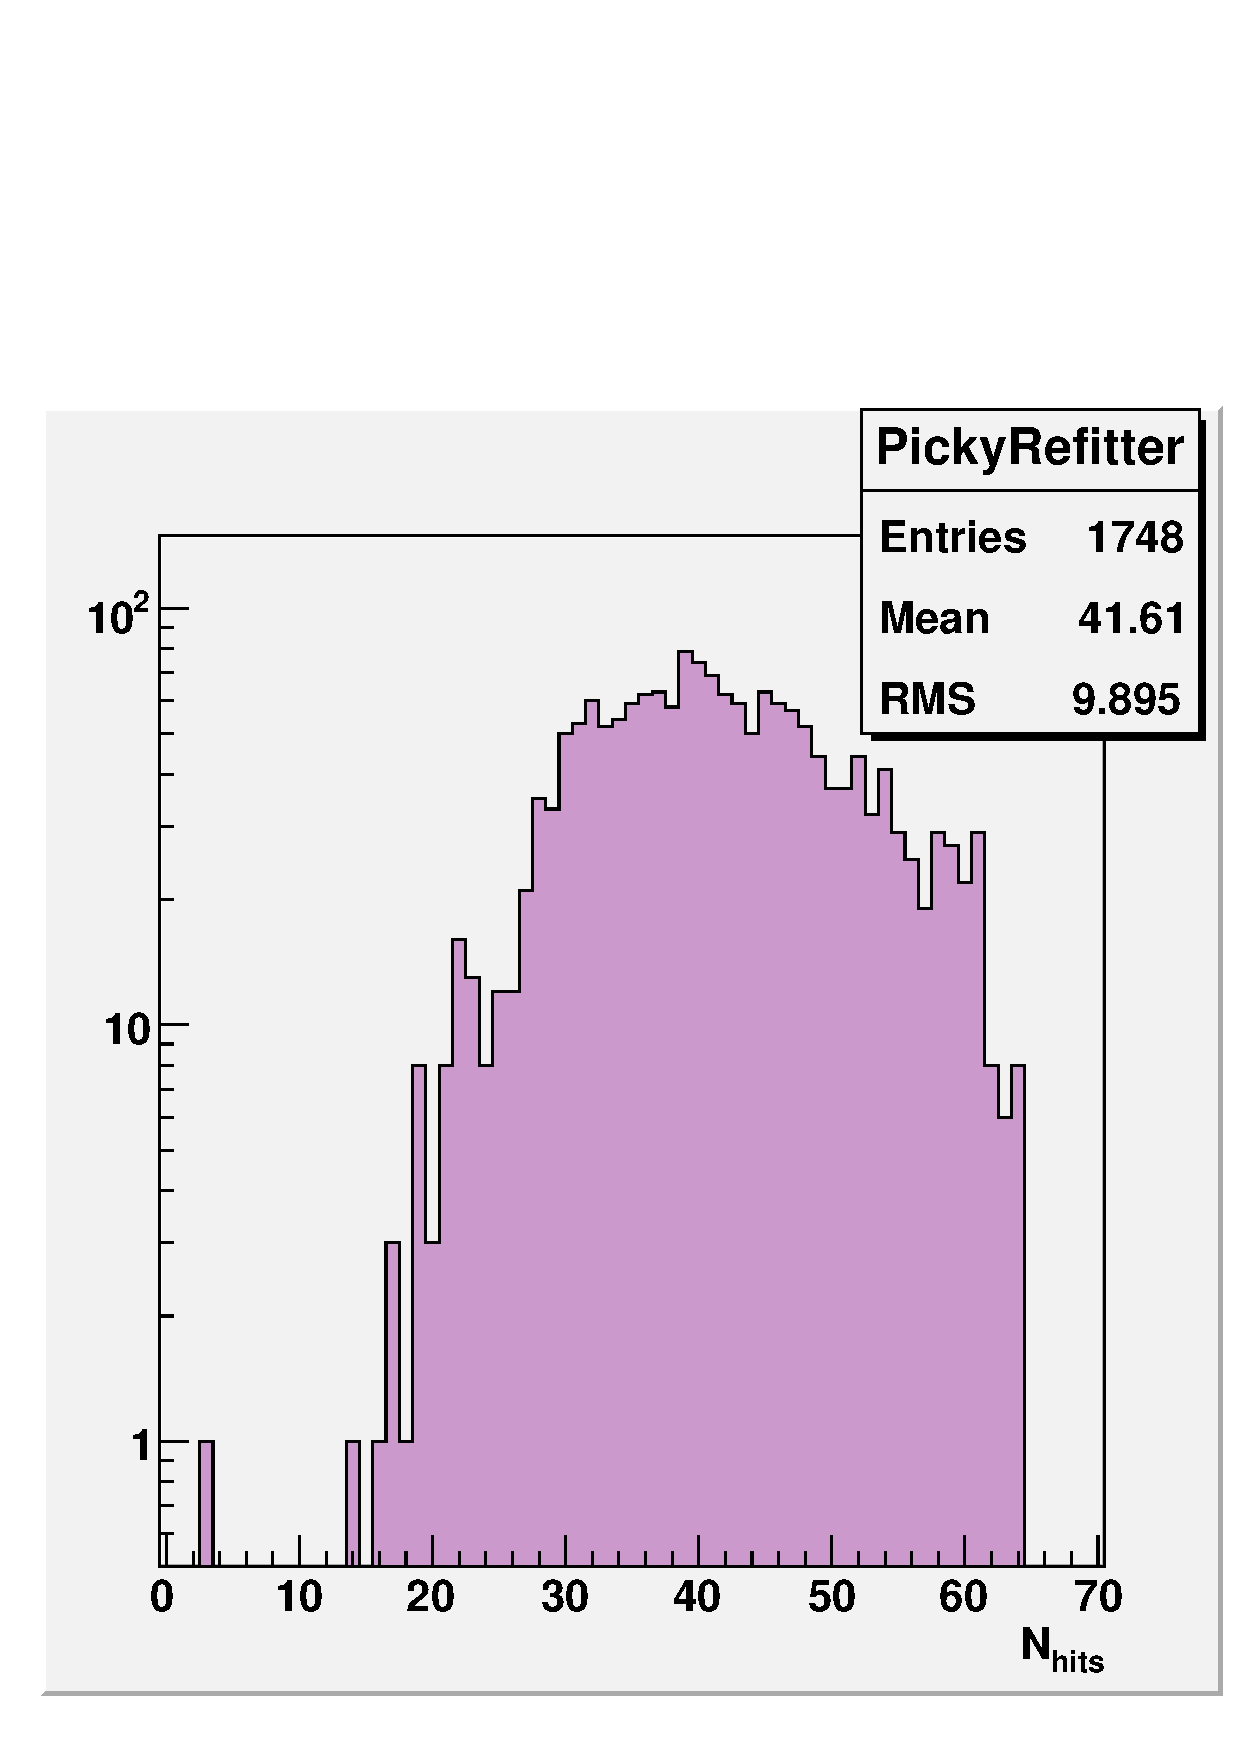
\includegraphics[width=\linewidth]{nhits_picky.pdf}
\column{0.5\linewidth}
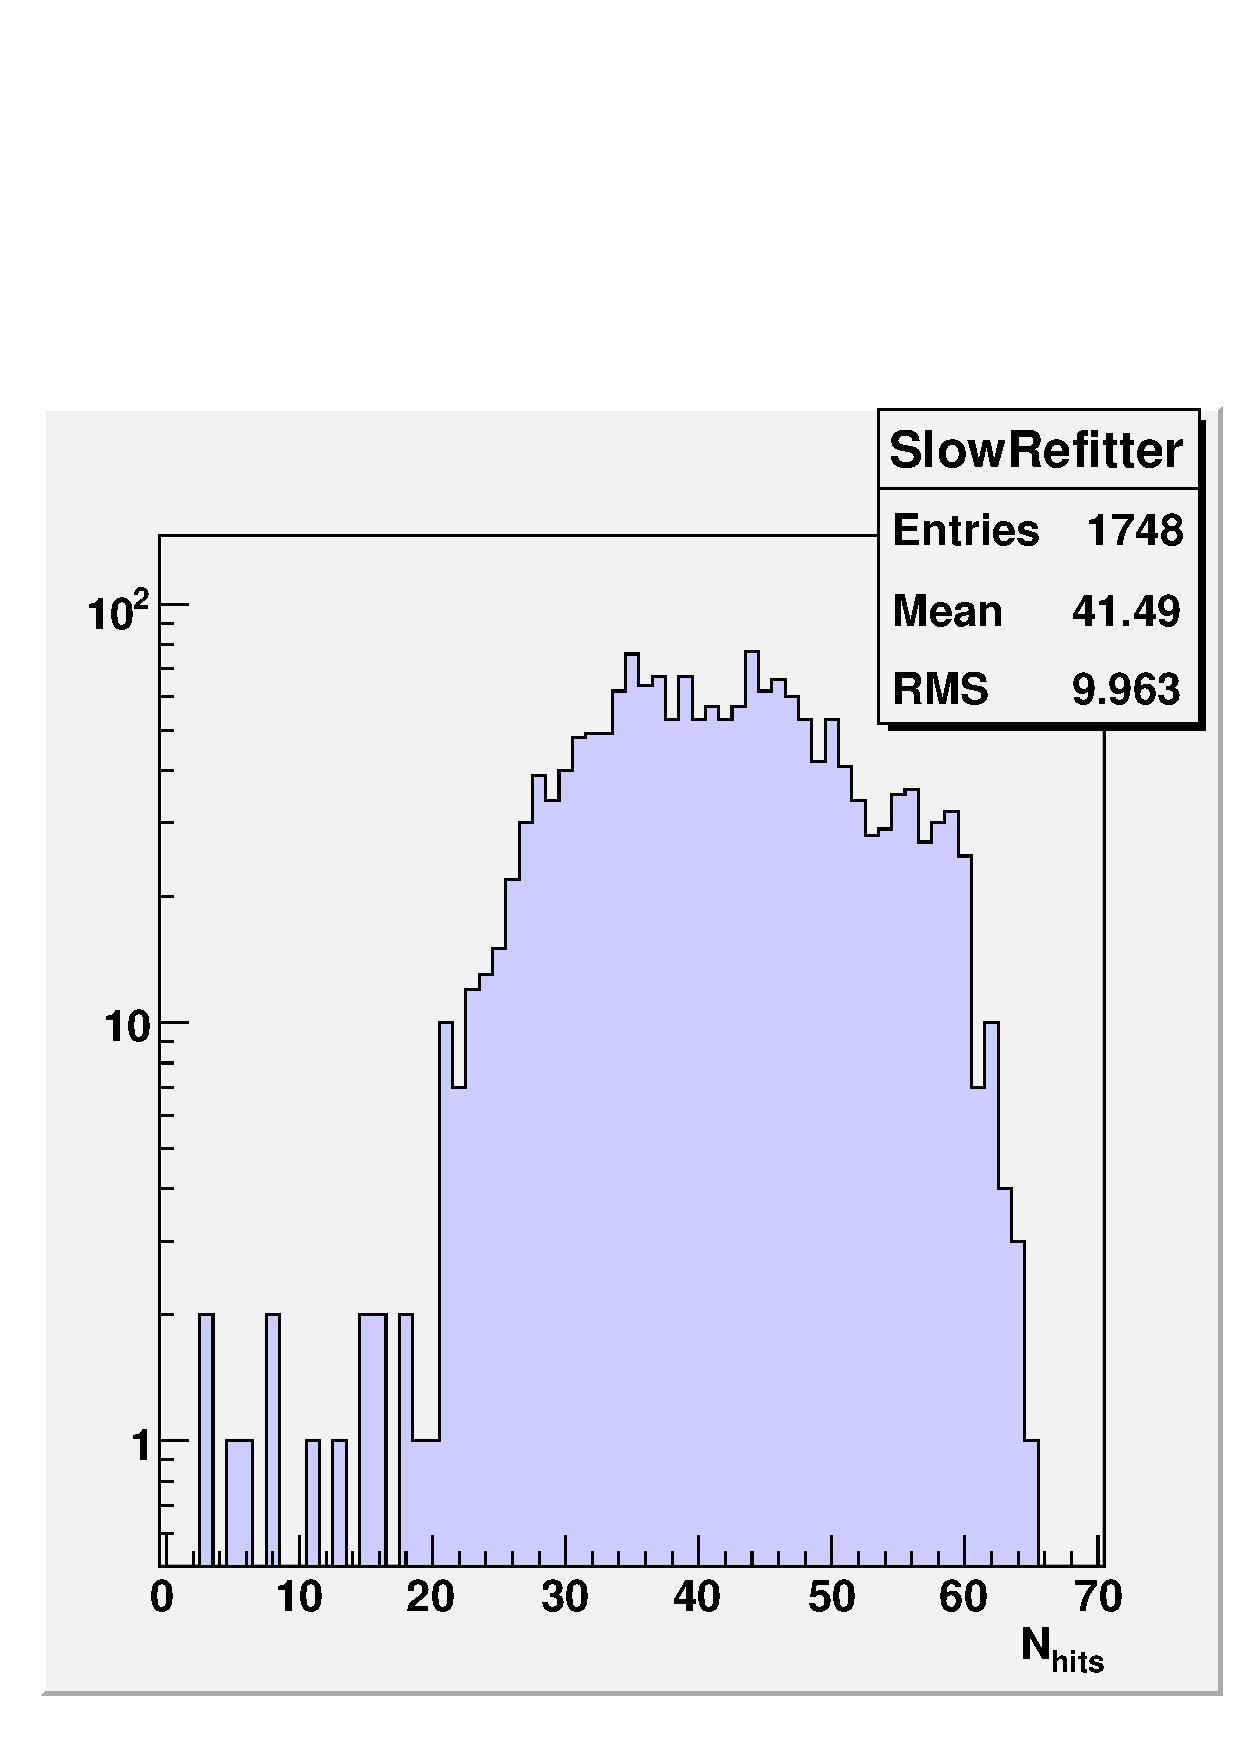
\includegraphics[width=\linewidth]{nhits_slow.pdf}
\end{columns}
\end{frame}

\begin{frame}
\frametitle{Performance tests: $p_T$}

\begin{itemize}
\item No impact on core of $p_T$ accuracy: 5.5\% in both cases
\item But it cleans up tails (could be relevant for Drell-Yan backgrounds)
\item Picky RMS: 20\% \hspace{0.1 cm} Slow RMS: 13\%
\end{itemize}

\vfill
\begin{columns}
\column{0.5\linewidth}
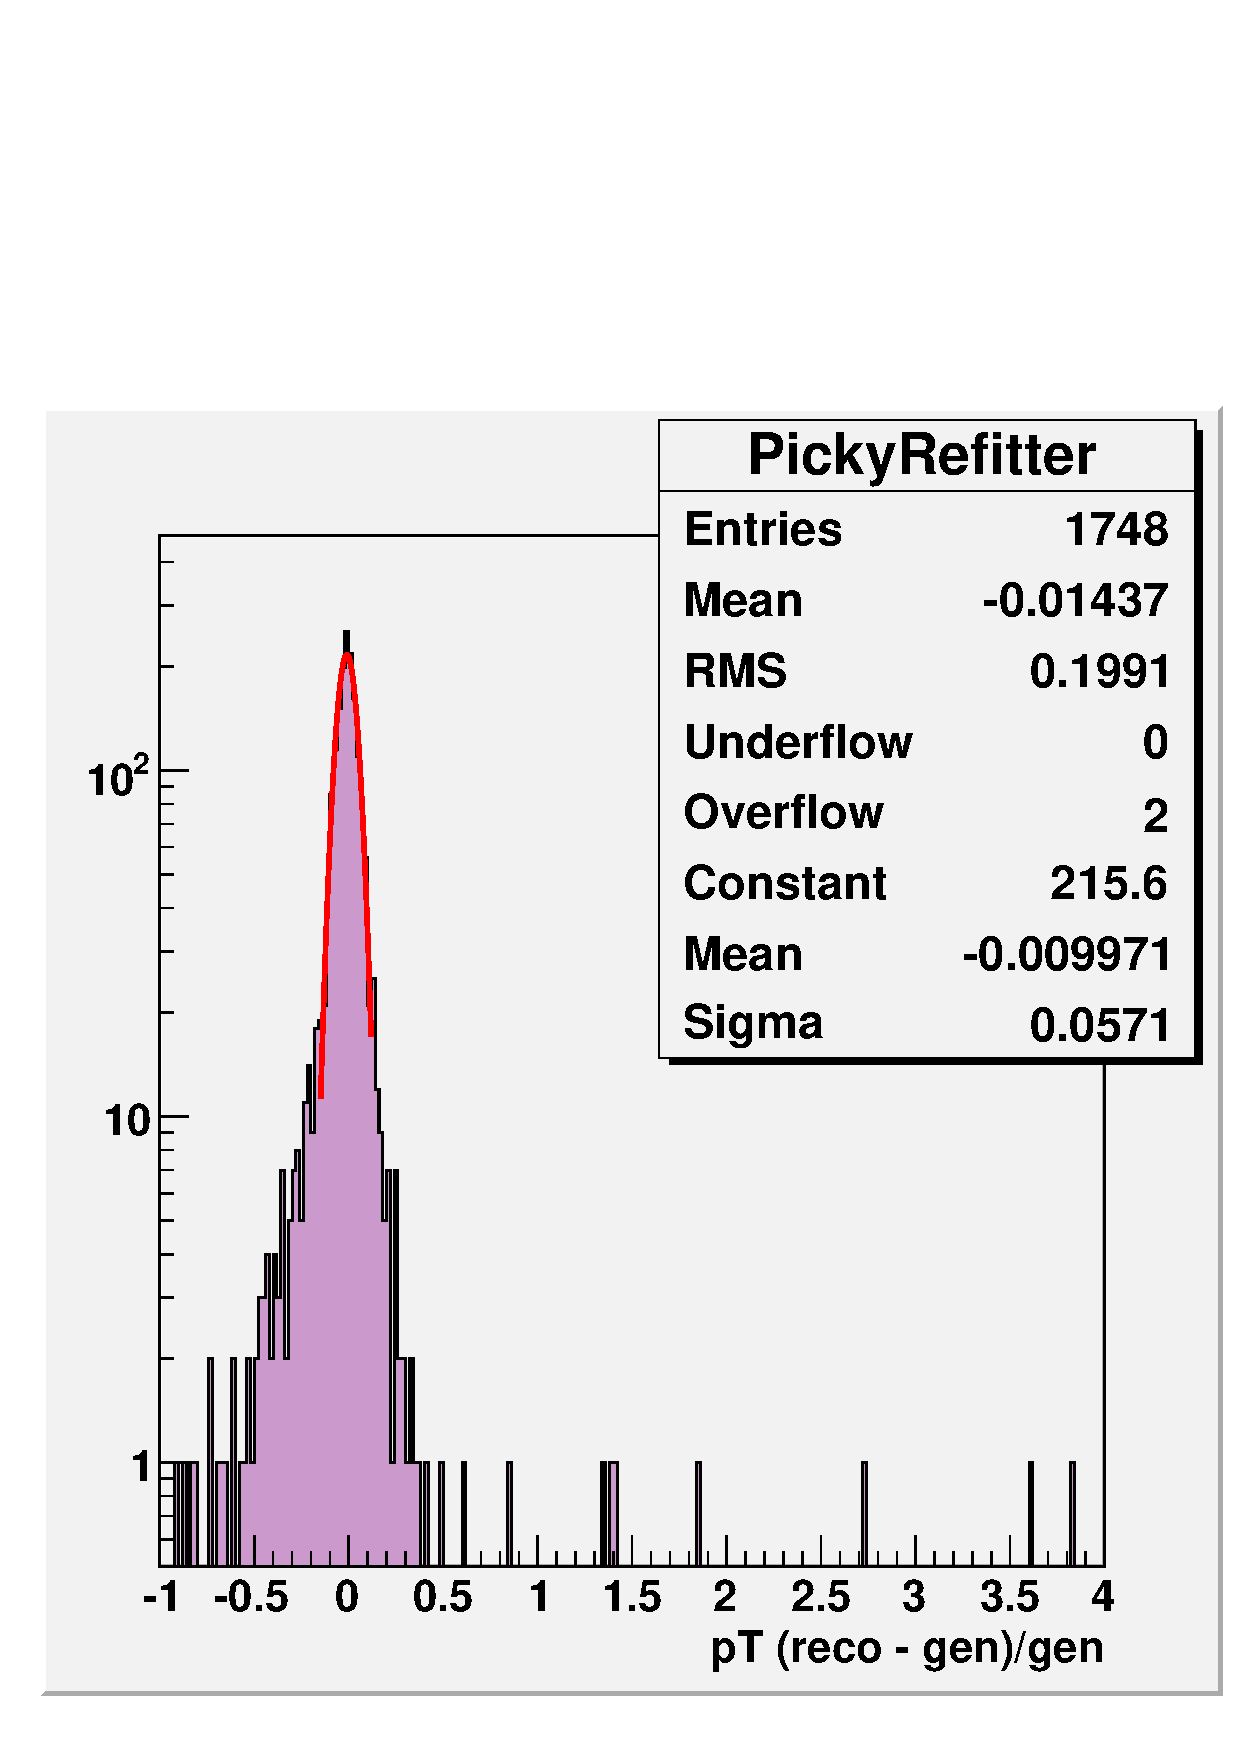
\includegraphics[width=\linewidth]{ptresolution_picky.pdf}
\column{0.5\linewidth}
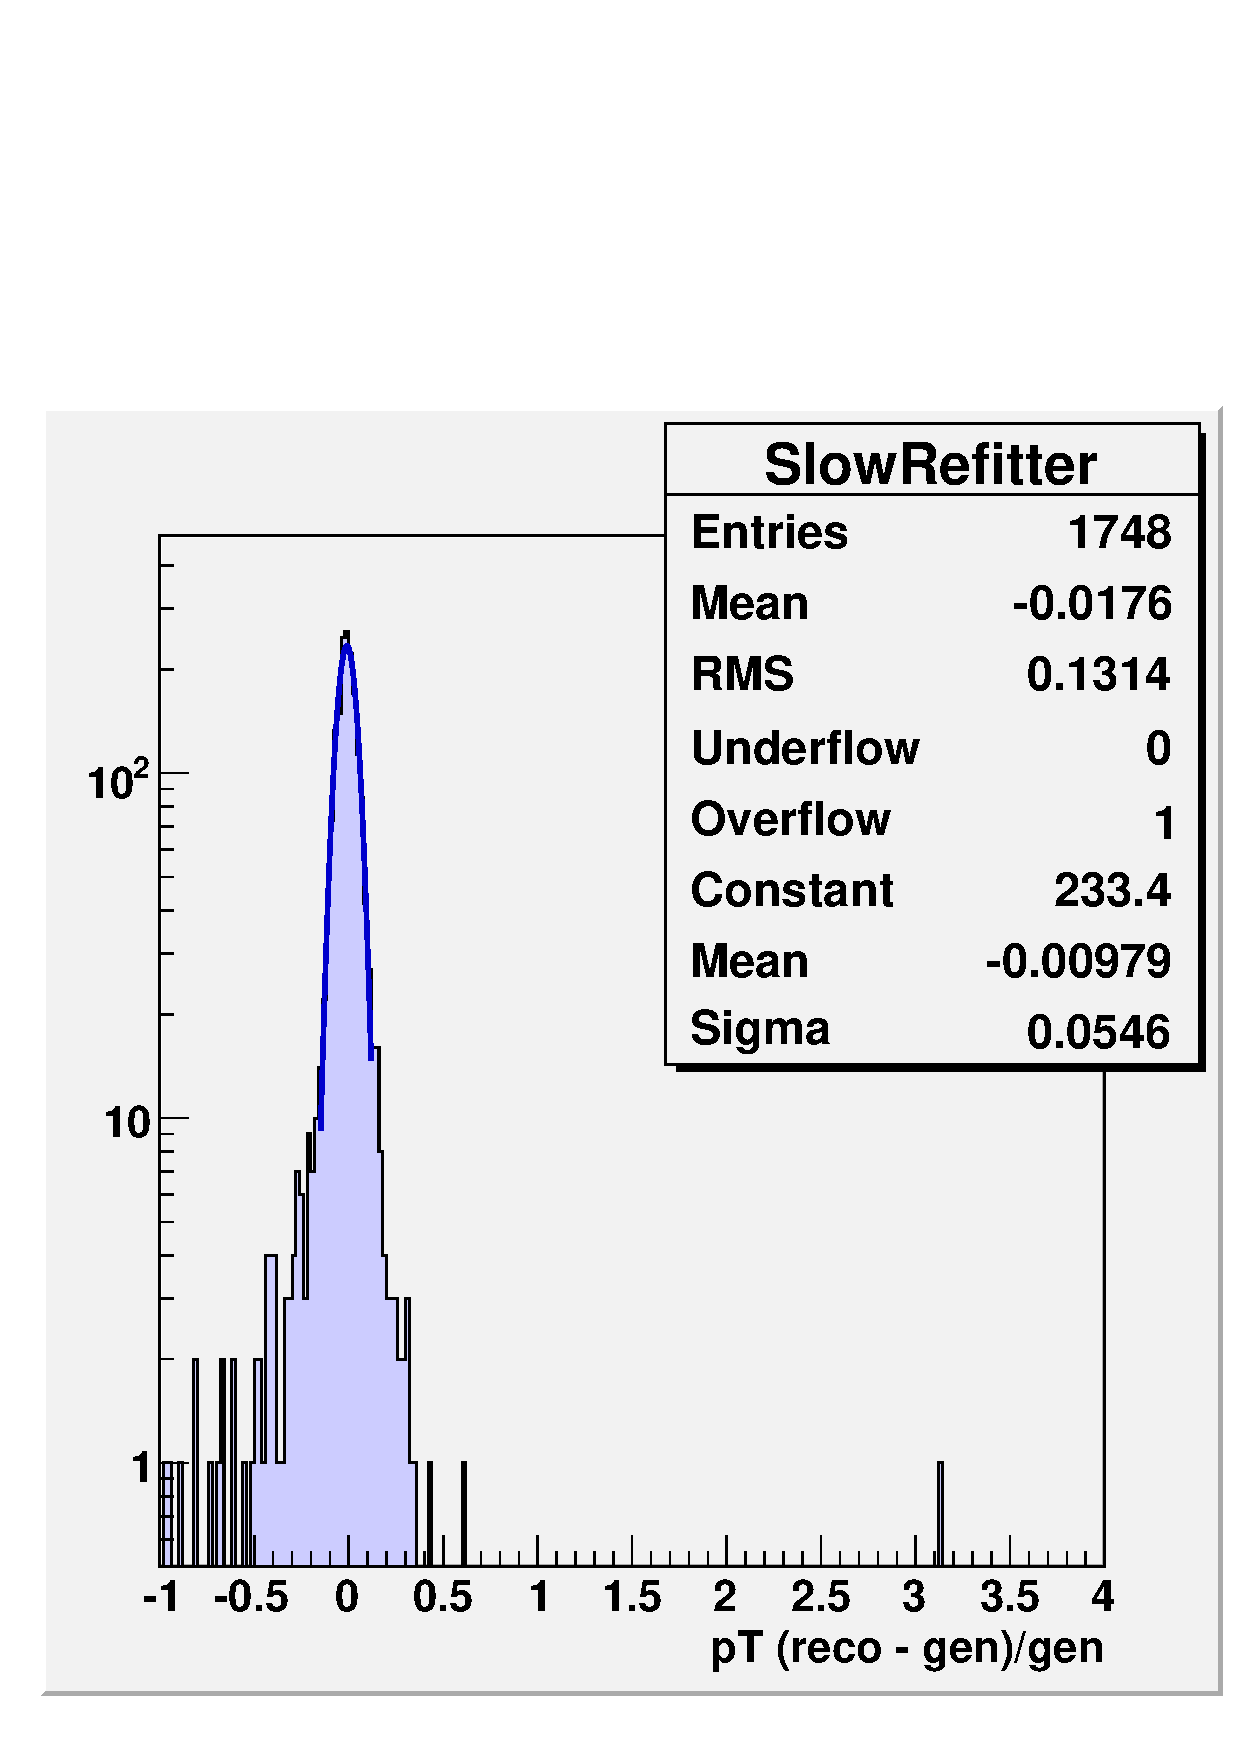
\includegraphics[width=\linewidth]{ptresolution_slow.pdf}
\end{columns}

\end{frame}

\begin{frame}
\frametitle{Another (possibly) useful cut}

\begin{itemize}
\item Pre-count number of hits on each chamber to exclude chambers with lots of showering
\begin{itemize}
\item more likely to pick up delta-ray hit if they are too dense
\end{itemize}
\item Presented cut values were used in this study (but not \mbox{chosen carefully!)\hspace{-1 cm}}
\end{itemize}

\vfill
\begin{columns}
\column{0.5\linewidth}
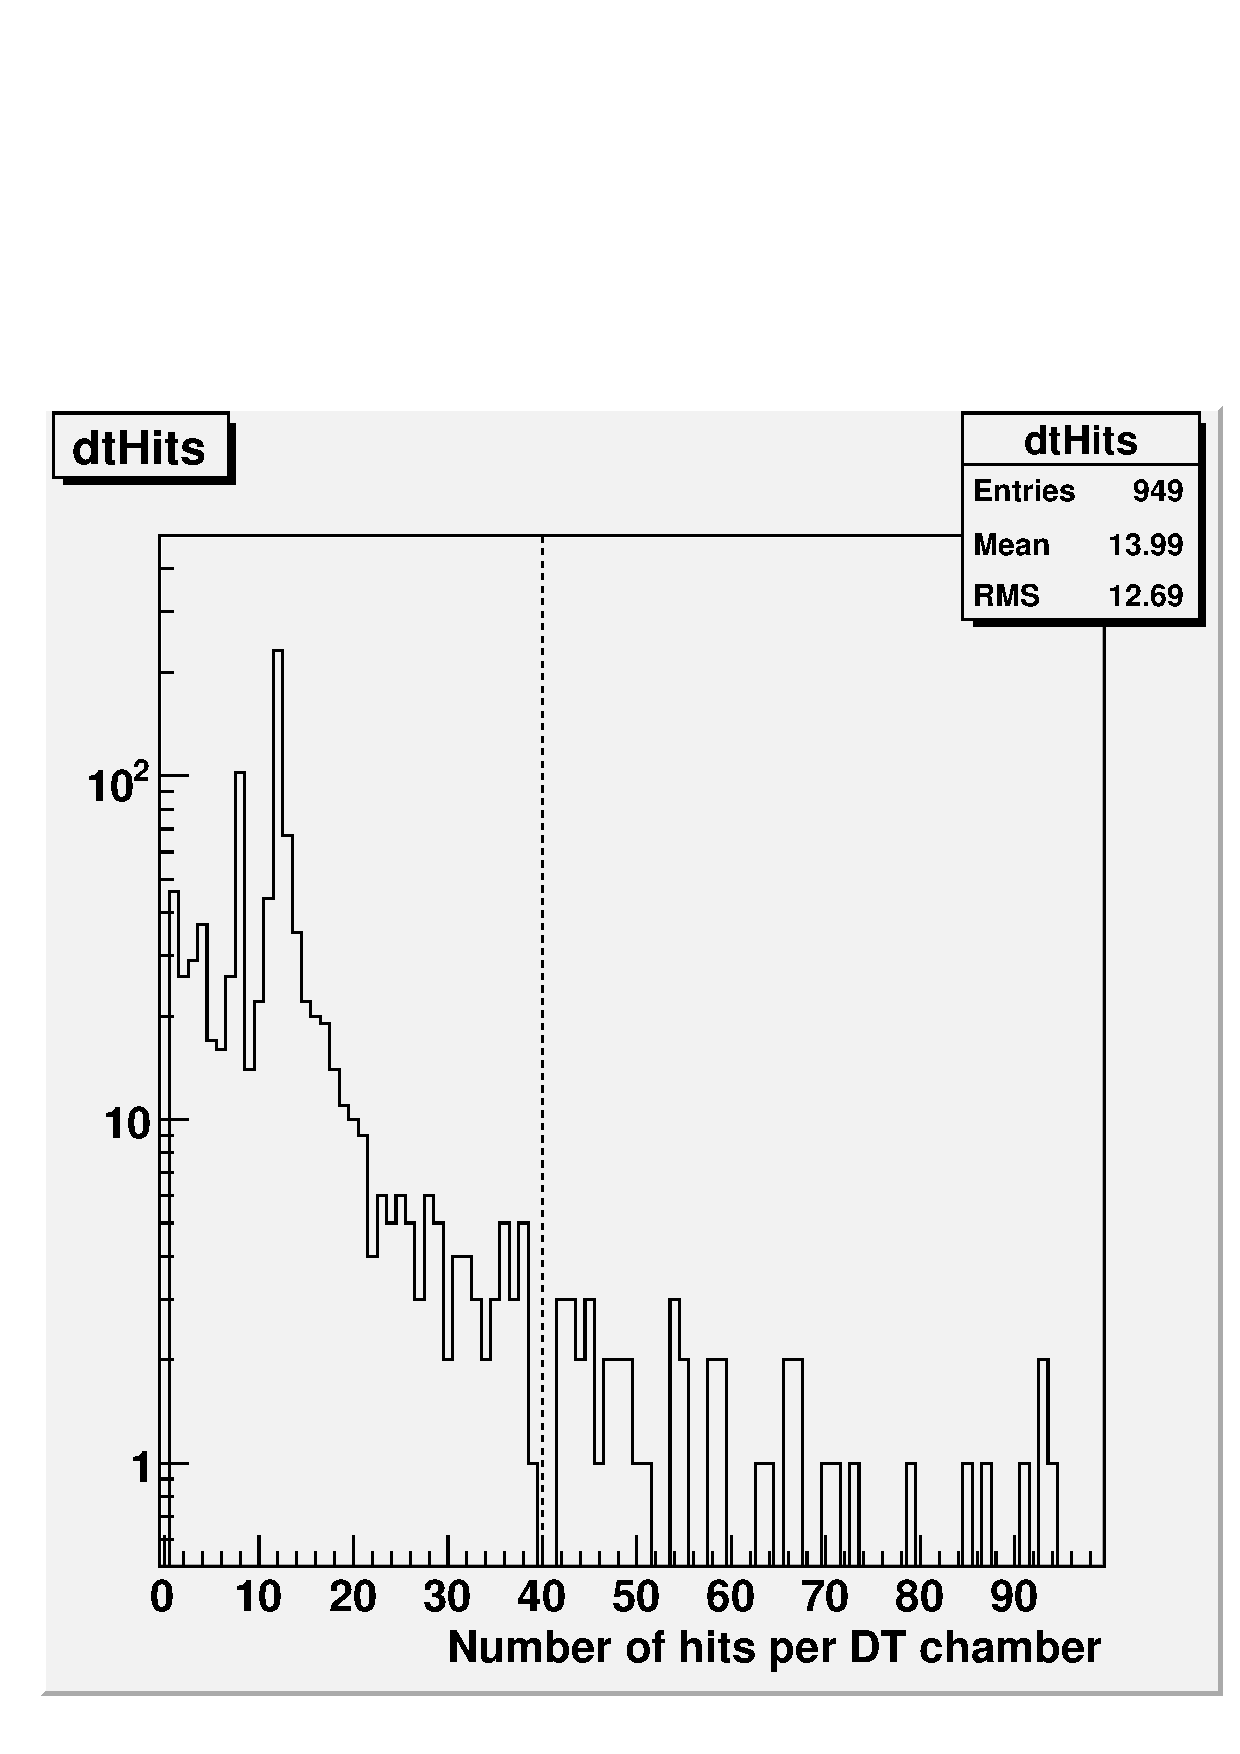
\includegraphics[width=\linewidth]{dtHits.pdf}
\column{0.5\linewidth}
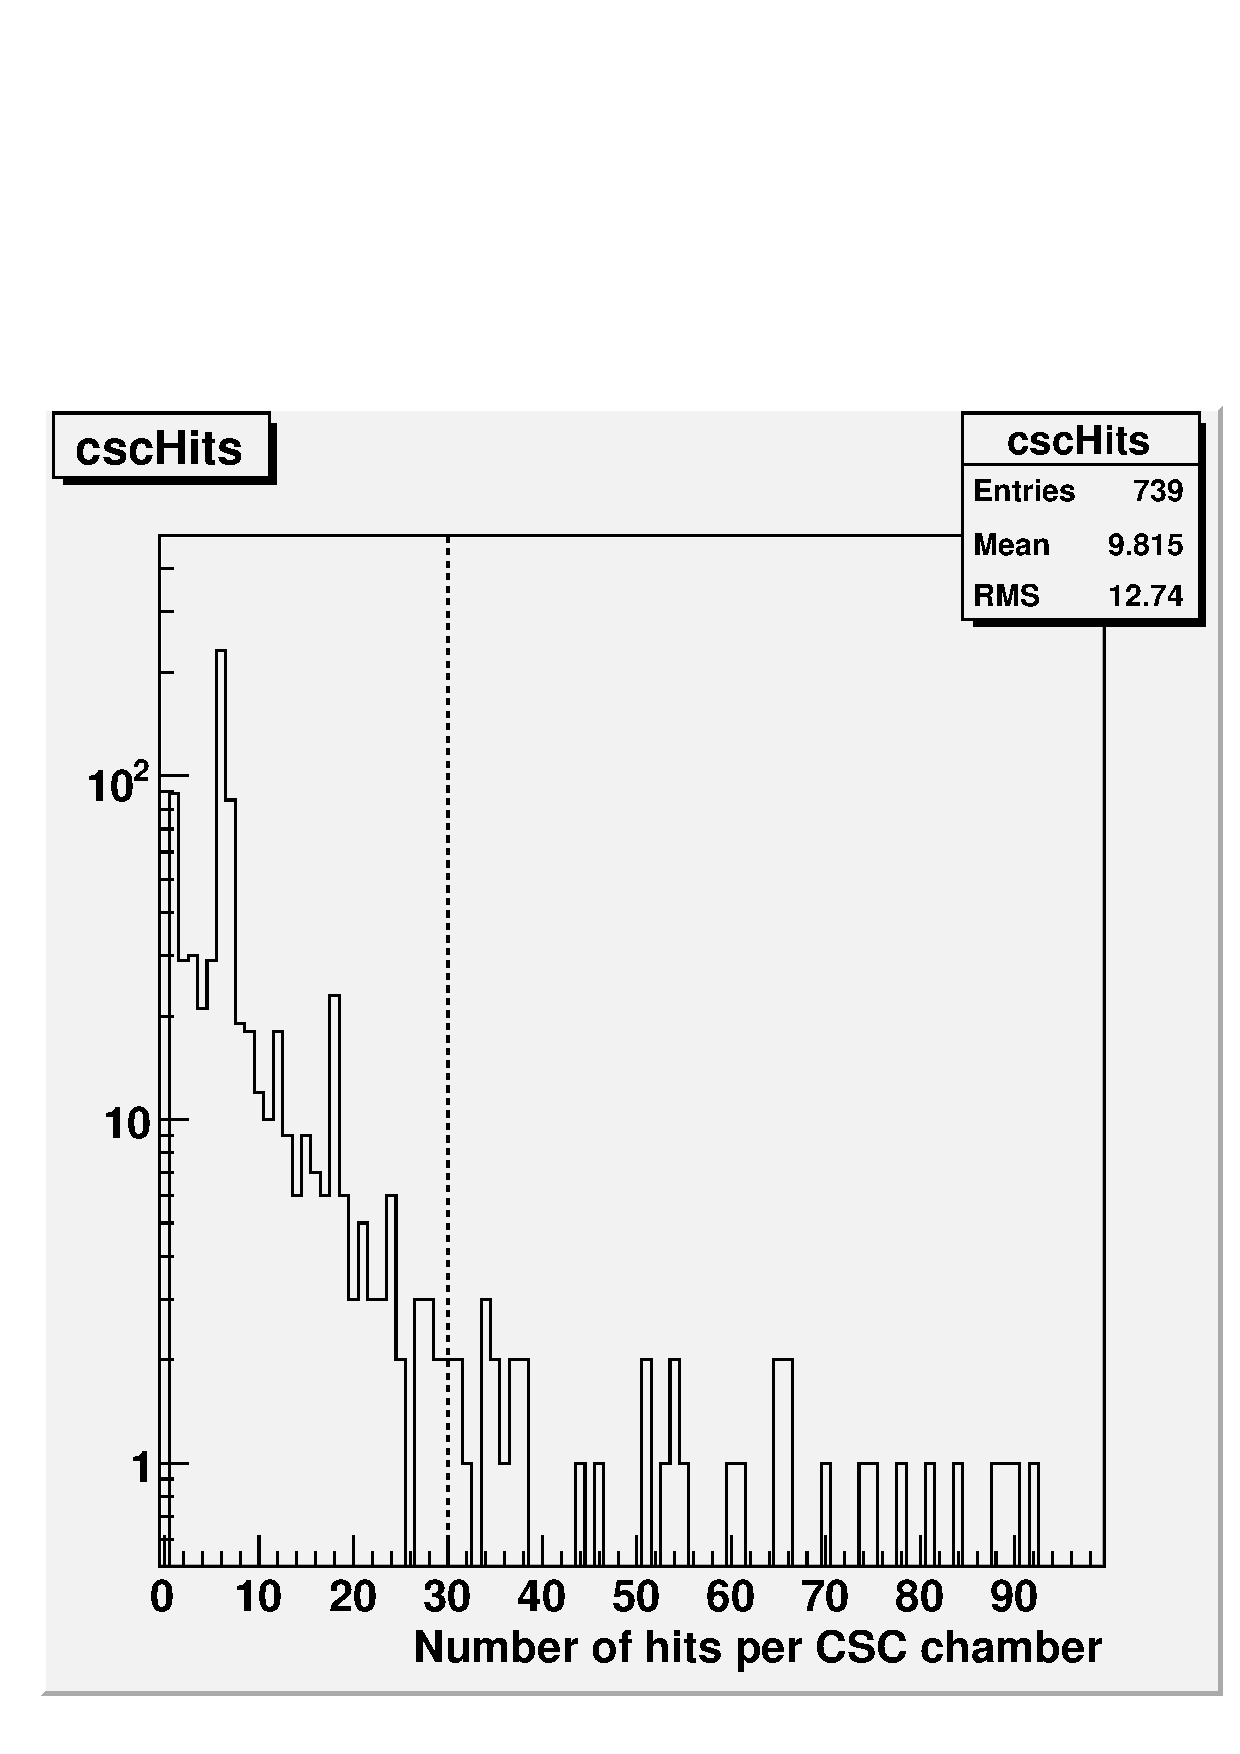
\includegraphics[width=\linewidth]{cscHits.pdf}
\end{columns}

\end{frame}

\begin{frame}
\frametitle{Evident need for more tuning}

\begin{itemize}
\item Computed probability of track $\chi^2$ from page 6 (should be flat)
\item Picky clearly has a tail of too-high $\chi^2$ which Slow refitter \mbox{mostly fixes\hspace{-1 cm}}
\item But Slow refitter also biases the central distribution toward \mbox{too-low $\chi^2$\hspace{-1 cm}}
\item Problem with (arbitrarily-chosen) value of missing hit penalty?
\end{itemize}

\vfill
\begin{columns}
\column{0.5\linewidth}
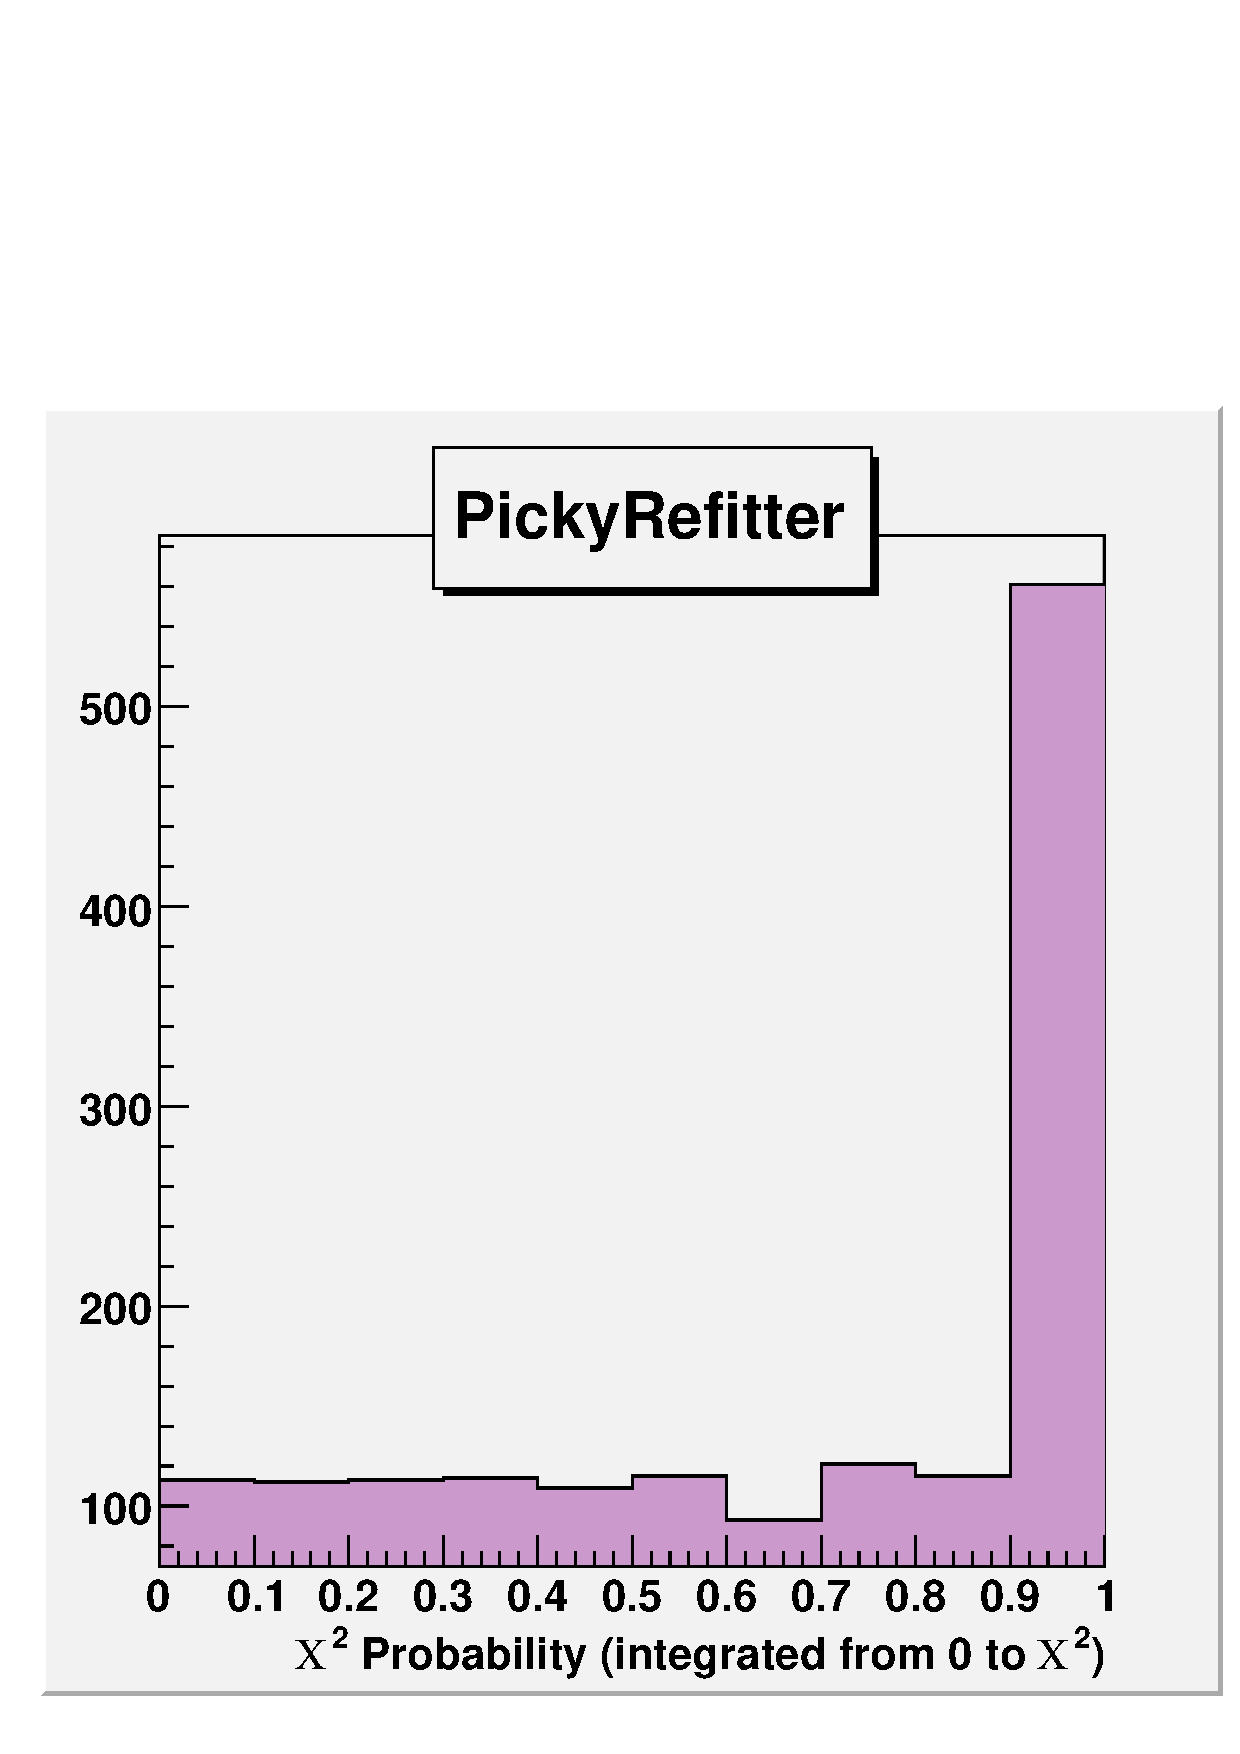
\includegraphics[width=\linewidth]{probability_picky.pdf}
\column{0.5\linewidth}
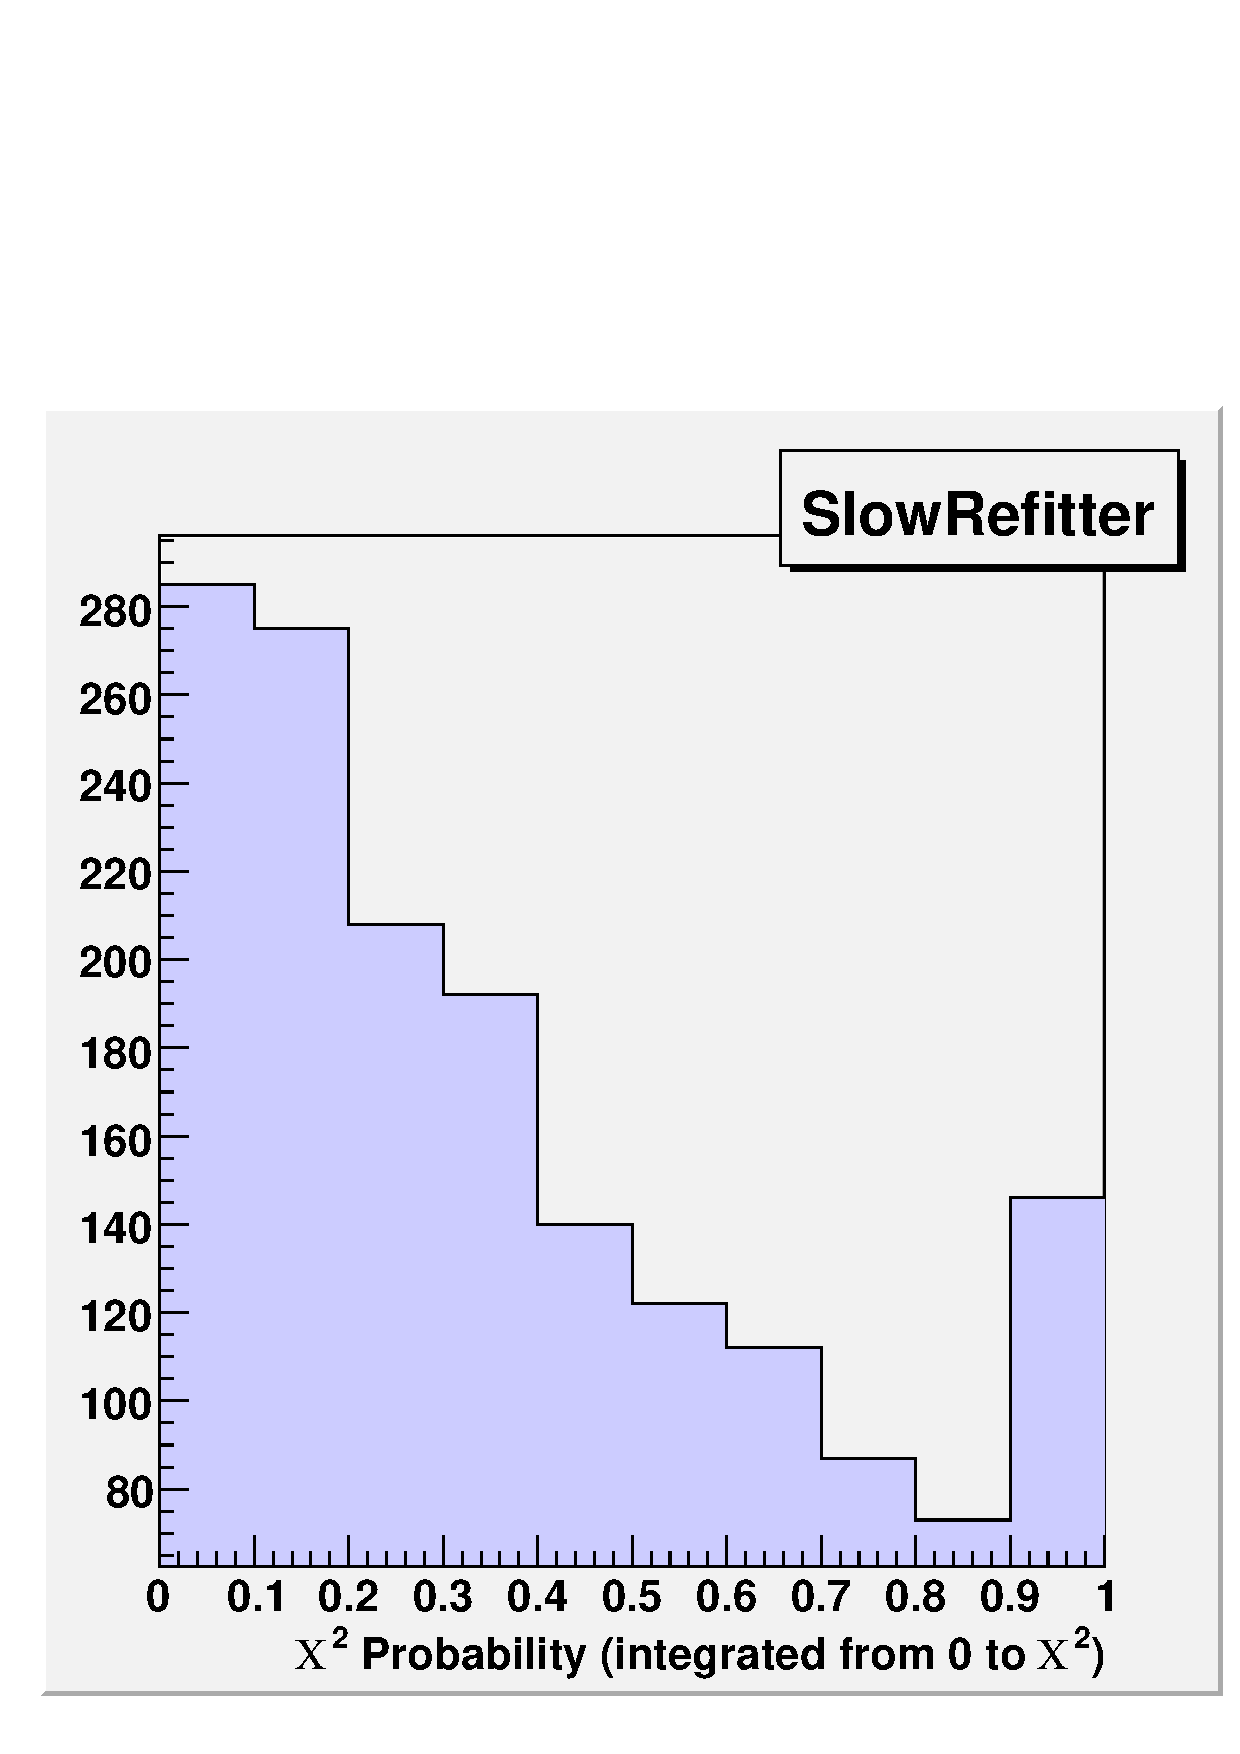
\includegraphics[width=\linewidth]{probability_slow.pdf}
\end{columns}

\end{frame}

%% \section*{First section}
%% \begin{frame}
%% \begin{center}
%% \Huge \textcolor{blue}{First section}
%% \end{center}
%% \end{frame}

\begin{frame}
\frametitle{Conclusions}
\begin{itemize}\setlength{\itemsep}{0.25 cm}
\item We can more carefully fit our best muons if we're willing to wait
\item Cleans up tails of distributions, but parameters need to be tuned
\end{itemize}

\vfill
\hspace{-0.83 cm} \textcolor{darkblue}{\Large Open questions}

\vspace{0.35 cm}
\begin{itemize}\setlength{\itemsep}{0.25 cm}
\item Is the $\chi^2$ distribution issue inherent to the method, or a
  function of the parameters?
\item Are these tracks stable under multiple refits (fixing the set
  of hits)?

\vspace{0.1 cm}
If so, perhaps it can provide insight into why GlobalMuons and
TeVRefittedMuons are not.
\end{itemize}
\label{numpages}
\end{frame}

\end{document}
